\newpage

\section{Simulation Analysis}
\label{sec:simulation}

In this section, we will the obtained results by simulating the referred circuit in Ngspice. 

In order to analyze the circuit and achieve the main goal of this laboratory assignment, we have developed an optimization ocatve algorithm that would give us the values which would leat to the greater merit value. The obtianed values were the following ones, presented in table \ref{tab:vsim1}:

\begin{table}[h]
    \centering
    \begin{tabular}{|l|c|}
    \hline
    {\bf Element } & {\bf Value} \\
    \hline \hline
    n (Transformer) & 15.70082452 \\
    \hline
    Number of diodes & 20 \\
    \hline
    C F & 3.3750e-05 F \\
    \hline
    Renvelope & 26k \\
    \hline
    Rregulator  & 10k \\
    \hline
    \end{tabular}
    \caption{Obtained values by optimization ocatve script}
    \label{tab:vsim1}
\end{table}

Then, using the expression given by the Professor, we can automatically compute the cost: 

\begin{equation}
    Cost = 72.15 
    \label{eq:Cost}
\end{equation}

The plots shown below are related to the variables $V_{input}$, $V_{envelope}$ and $V_{output}$ in function of time. Those were a result of the analysis in Ngspice. The values for the merit, ripple and average output voltage are in table \ref{tab:tsim1}.

\begin{figure}[!ht] \centering
\caption{Envelope detector voltage}
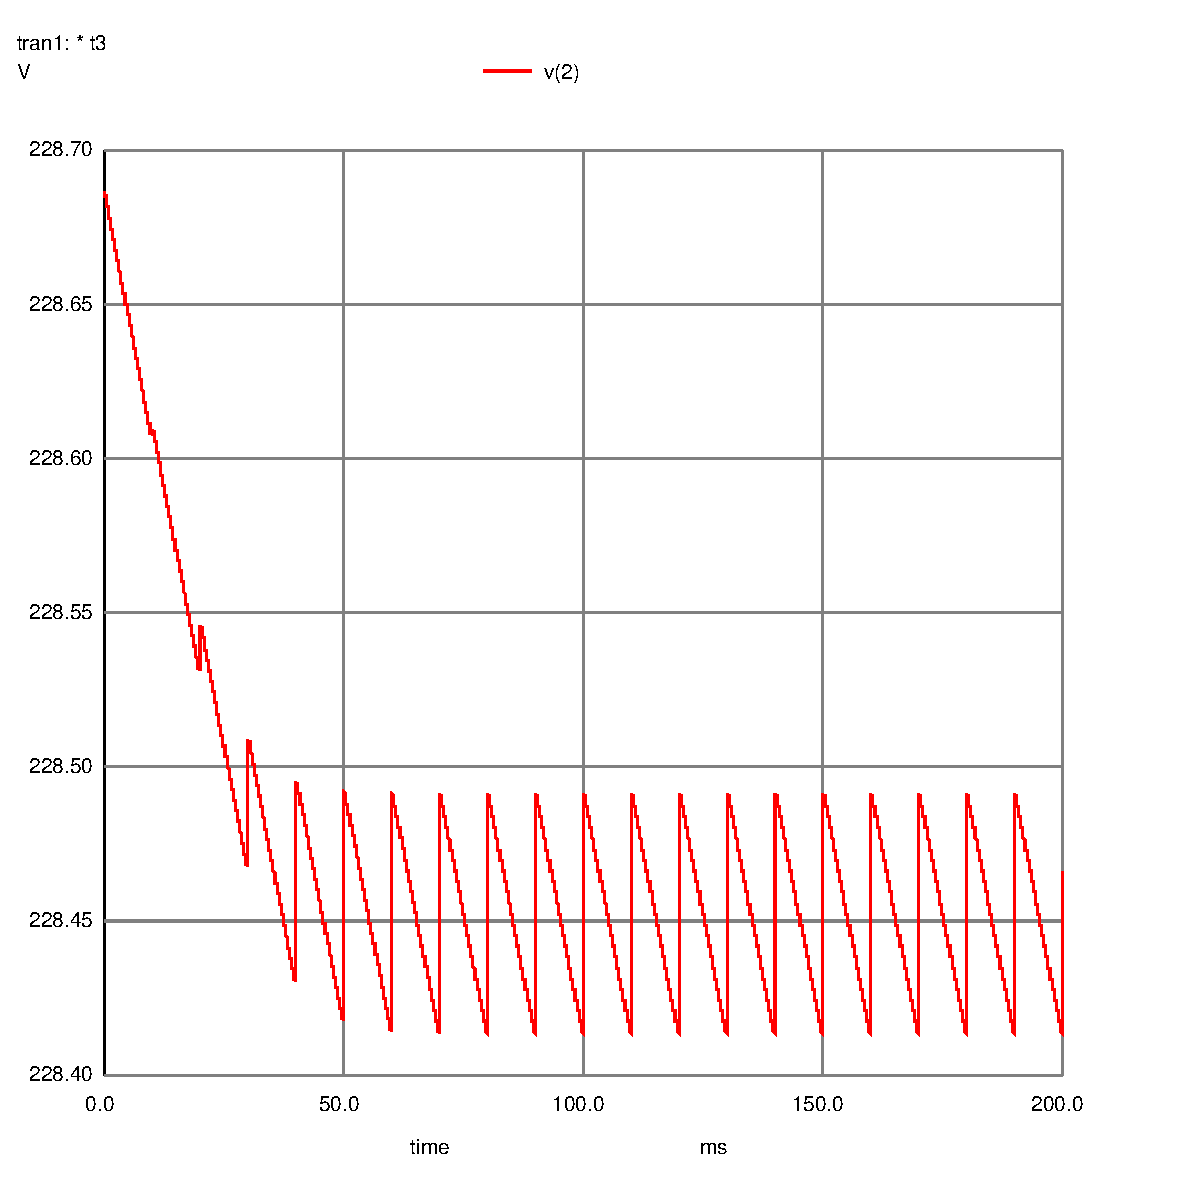
\includegraphics[width=0.6\linewidth]{venv.eps}
\label{fig:gteo1}
\end{figure}

\begin{figure}[!ht] \centering
\caption{Output voltage and Output voltage - 12 V}
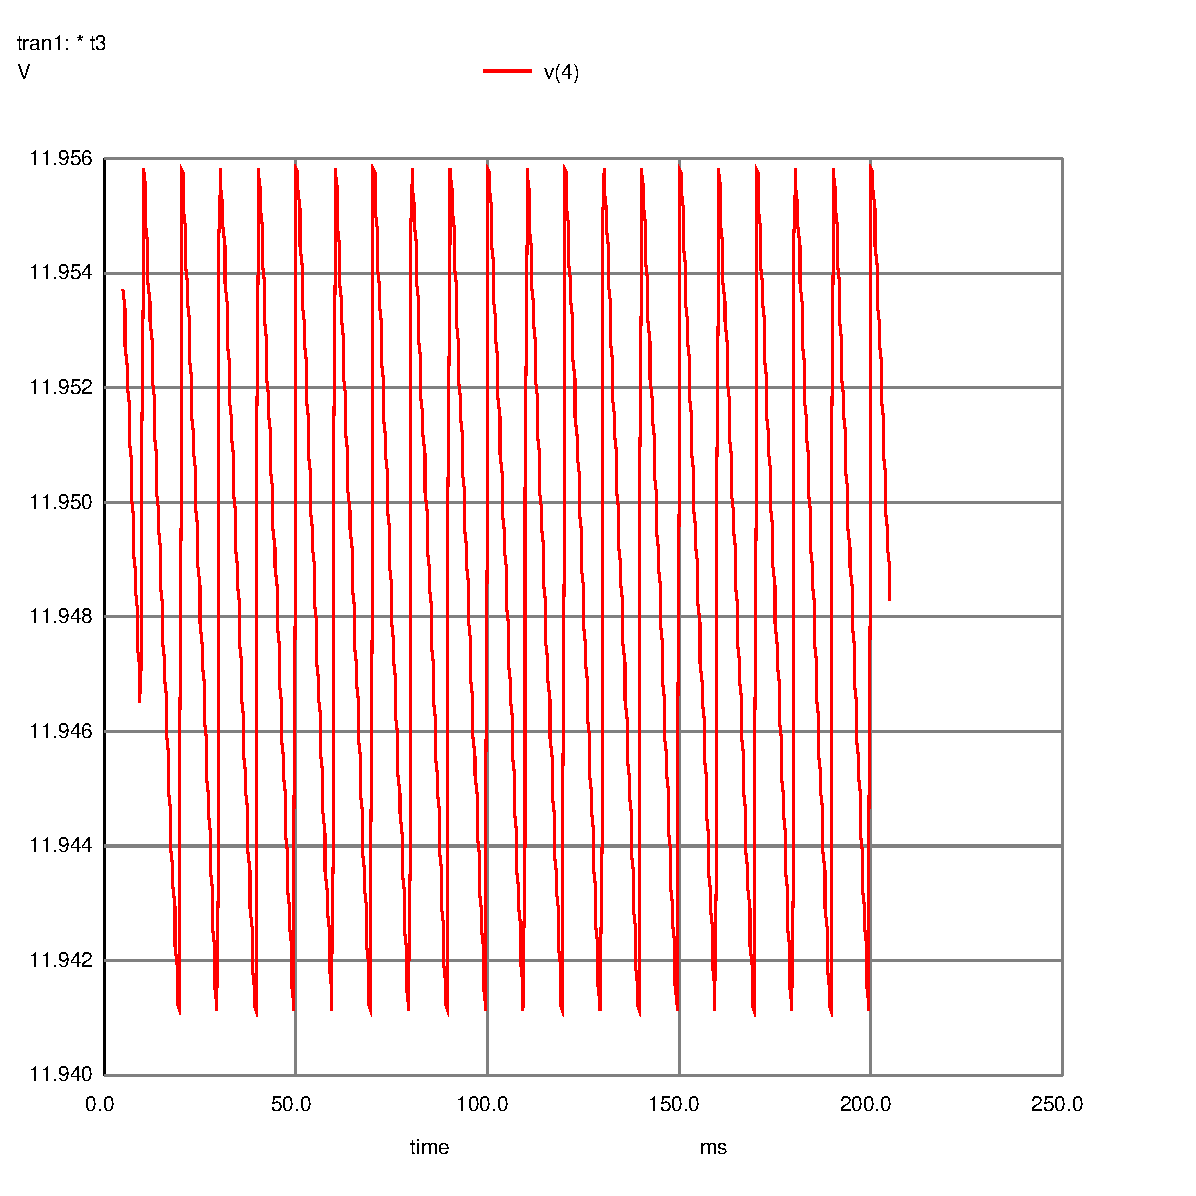
\includegraphics[width=0.45\linewidth]{vout.eps}
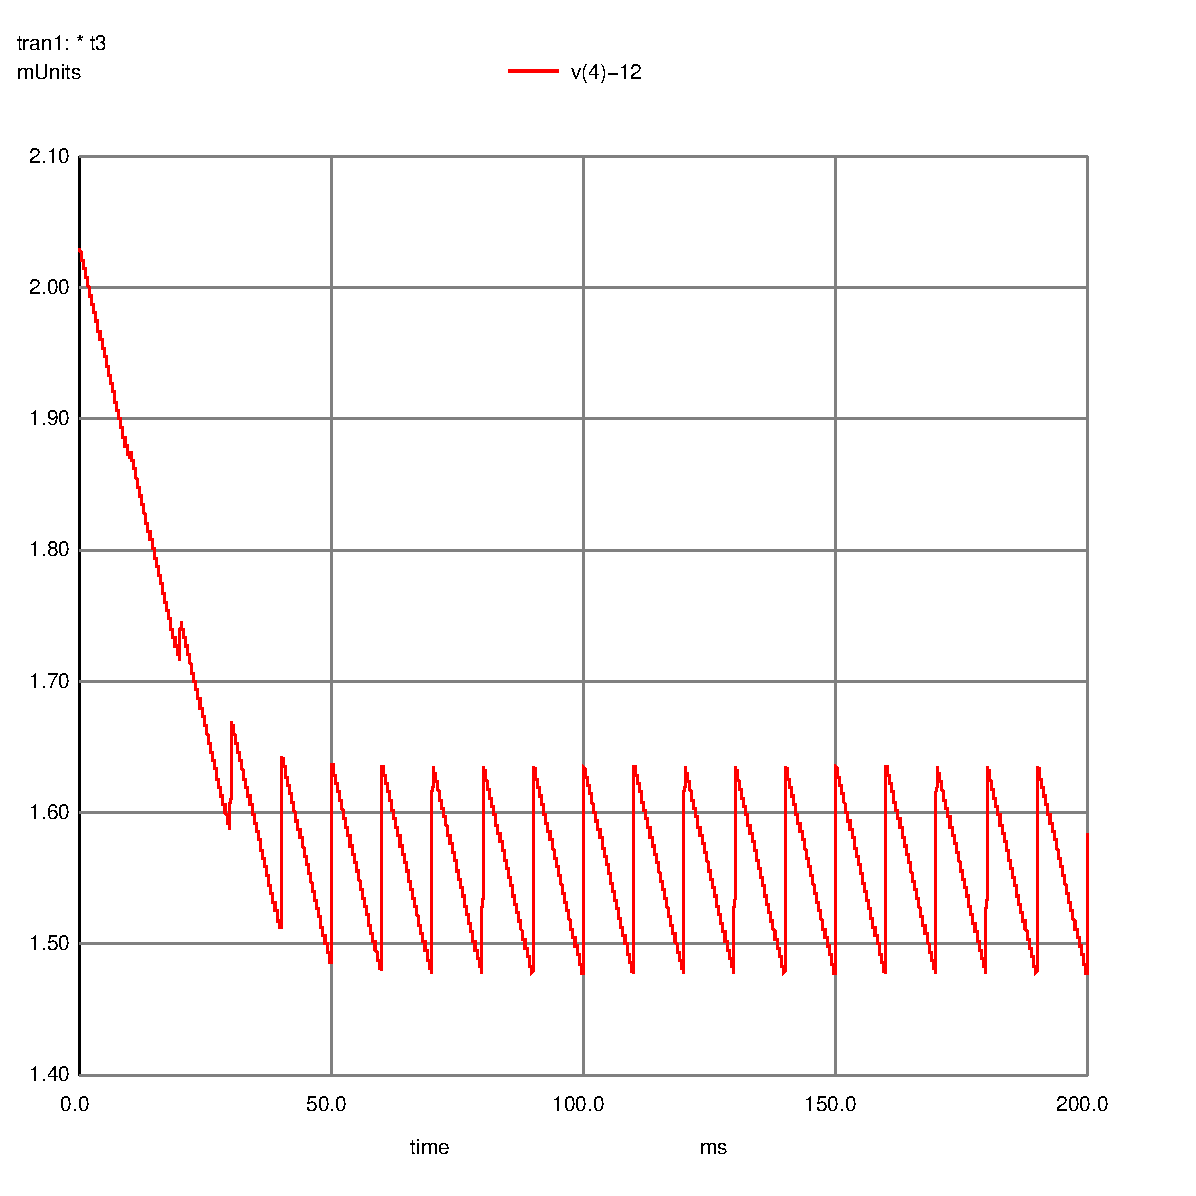
\includegraphics[width=0.45\linewidth]{vout(ac+dc).eps}
\label{fig:gteo2}
\end{figure}


\begin{figure}[!ht] \centering
\caption{Input, Envelope and Output voltages}
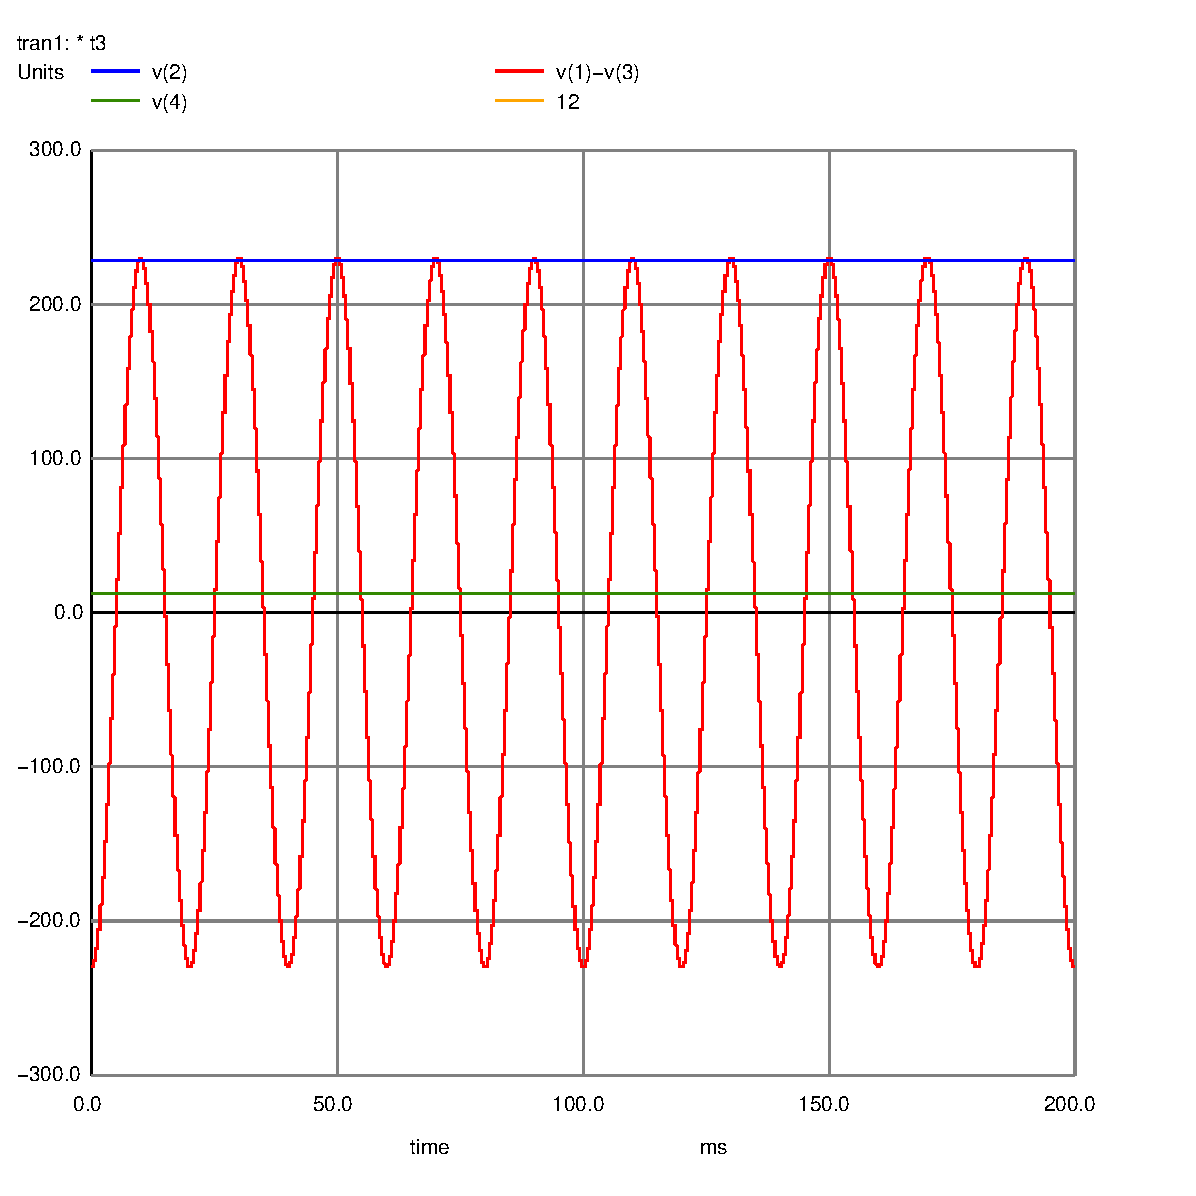
\includegraphics[width=0.6\linewidth]{vs_vout.eps}
\label{fig:gteo4}
\end{figure}

\begin{table}[h]
    \centering
    \begin{tabular}{|l|c|}
    \hline
    {\bf Element } & {\bf Value } \\
    \hline \hline
    Average Output Voltage [V] & 1.199998e+01 \\  
    \hline
    Output Voltage Ripple [V] & 7.809000e-02 \\
    \hline
    Merit &  1.774688e-01 \\
    \hline
    \end{tabular}
    \caption{Simulation Values for Average, Ripple and Merit.}
    \label{tab:tsim1}
\end{table}







